\documentclass[12pt]{article}
\usepackage[utf8]{inputenc}
\usepackage{amsmath}
\usepackage{graphicx}

\title{ISP - The Traffic Light System}
\author{Joshua Liu}
\author{TEJ 3M1 - Mr.Wong}
\date{\today}


\begin{document}
\maketitle
\begin{center}
    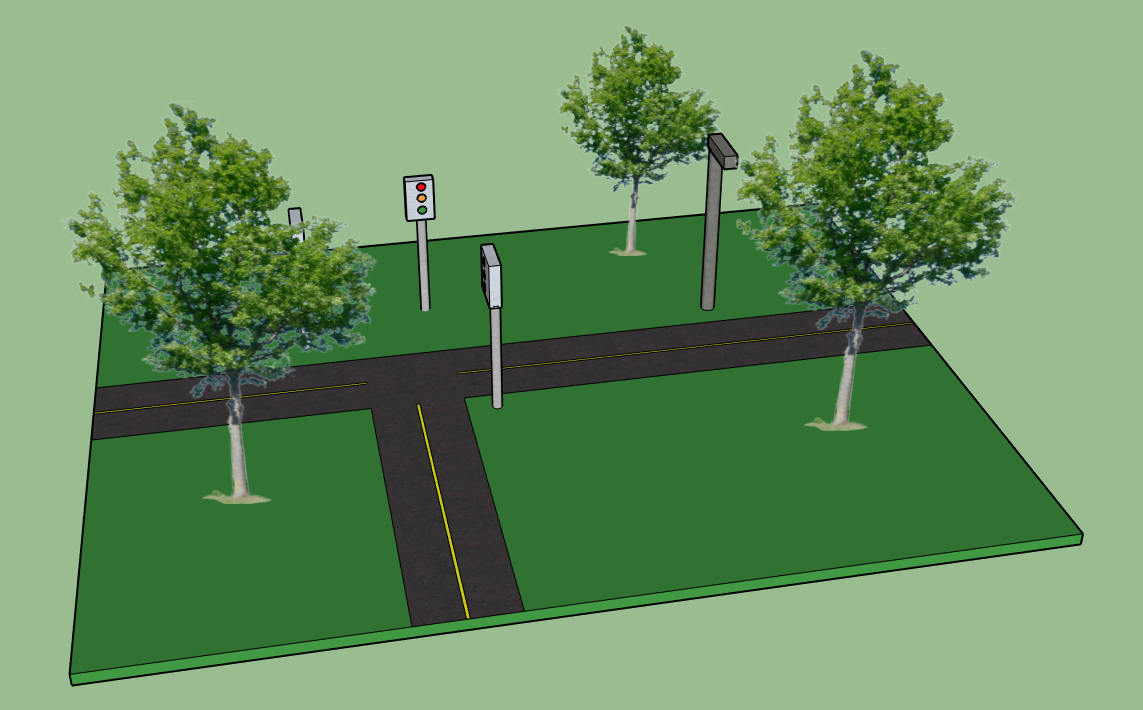
\includegraphics[scale=0.3]{Sketchup.PNG}
\end{center}

\section{Sketchup Drawing}

In the image above, we created a model intersection with traffic lights, street light, lanes, and trees. Most models were built by hand using primative shapes such as rectangles and circles, while objects like trees, which contain more complex details, were imported from Sketchup's 3D Warehouse.

\section{Challenges}

Some challenges in creating a working traffic light system was the code, more specifically delay and timing. One feature of this traffic light system is to have a gate with a ultrasonic sensor, the gate stays open when a car is between 150 cm and 200 cm away from the gate and stays within that range for 3 seconds, the gate would open and stay open for 1 second. The challenge was to keep the gate open for a second without using delay(), as that would stop the entire system. One workaround I found was do use a global variable, which would track the time at which the gate opened, and we can insert an if statement one the difference between the current time and the variable's time is greater than 1 second, close the gate.

\medskip
Another challenge was designing the model in Sketchup. I had difficulty getting used to the web UI as the controls were different from other 3d modeling websites such as Tinkercad. Although, tutorials helped and I understood the UI after about half an hour. I also had difficulty with the Sketchup tools, models would move in the wrong axis, models would "stick together", and the tool I was using would switch to a different tool. Luckily I was able to undo any mistakes I made with Ctrl-Z.

\section{Investigation}

The plan for the traffic system was for it to be created out of cardboard, styrofoam, glue, and the electronic components. I would use different types of paint so I could match the real model as close as possible to the Sketchup model. The cardboard would be used for the base of the model and any small models, such as the traffic light, the street light, and the gate, would be created out of styrofoam to keep it light but still maintain a shape.

The electronics of the system are broken down into four parts, the traffic lights, the street light, the gate, and the pushbutton.

The traffic lights mimic similar to real world traffic lights, the ones opposite flash green, yellow, and red then alternate to the two, or in this case one, traffic light in between. For each sequence, the traffic lights turn green for 3 seconds, and yellow for 2 seconds.

The street light take use of a photoresitor. The Arduino reads the signal produced by the photoresistor and would turn on the street light (led) when the signal becomes weaker, meaning it is getting darker.

The gate uses a similar idea and the street light, an ultra sonic sensor would detect when an object is between 150 cm and 200 cm away from it and turn the servo to open the gate when the object is within that range for 3 seconds, the servo will stay open for 1 second.

The pushbutton acts as a setting speed for the traffic lights, the pushbutton would increase the speed of the traffic light by a factor of 1 to 4, depending of the setting. The default is 1.

\section{Evaluation}
I think my project turned out well, I am glad in the effort I put in my project. If we could do this again, I would like to implement my ideas and build the model in the real world.

\end{document}